\chapter{Blockchain nell'era quantistica}
La Blockchain è indiscutibilmente una delle tecnologie più recenti e fiorente degli ultimi dieci anni, se non la tecnologia del futuro. Però a minacciare la sicurezza di quest'utlima è l'ormai incombente crescita di un ulteriore tecnologia: il Quantum Computing.

In particolare, algoritmi quantistici come l'\textit{algoritmo di fattorizzazione di Shor} e l'\textit{algoritmo di ricerca di Grover}, che sono alla base dell'odierna Blockchain, possono risolvere alcuni problemi in tempi considerevolmente minori rispetto alle loro controparti tradizionali, dando quindi la possibilità di violare, utilizzando migliaia di qubit, schemi di crittografia a chiave pubblica, come \textit{RSA} ed \textit{Elliptic Curve}, essenziali per la sicurezza della Blockchain. Nel 2015, infatti, il \textit{National Institute of Standards and Tecnology (NIST)} degli Stati Uniti ha dichiarato che la tecnologia quantistica ha il 15\% di probabilità di rompere lo schema crittografico RSA 2048 entro il 2026 e il 50\% di possibilità che ciò avvenga entro il 2031, ma che, entro il 2035, sarà sufficientemente avanzata per romperlo definitivamente \cite{mosca2018cybersecurity}.

Una soluzione a questo problema è la \textit{Post-Quantum Cryptography (PQC)} che ha come scopo quelllo di sviluppare dei sistemi crittografici in grado di resistere ad attacchi provenienti da computer quantistici e classici, e che allo stesso tempo si interfaccino con le attuali reti e protocolli di comunicazione. A partire da questo, il NIST ha iniziato un processo di ricerca, valutazione e standardizzazione di uno o più algoritmi di crittografica QR\footnote{Quantum Resistant, o resistente agli attacchi quantistici.} \cite{quantum_NIST}.

\section{Crittografia post-quantistica}
In crittografia, la \textbf{crittografia post-quantistica} (talvolta definita anche \textbf{quantum-resistant}) si riferisce ad algoritmi crittografici (solitamente algoritmi a chiave pubblica) che si ritiene siano sicuri contro un attacco crittoanalitico da parte di un computer quantistico. Come anticipato, il problema degli algoritmi attualmente in uso è che la loro sicurezza si basa su uno dei tre problemi matematici più difficili: il problema della fattorizzazione dei numeri interi, il problema del logaritmo discreto o il problema del logaritmo discreto a curva ellittica.

\subsection{Algoritmi}
Attualmente la ricerca sulla crittografia post-quantistica si concentra principalmente su sei diversi approcci:
\begin{description}
  \item[Crittografia basata su reti euclidee] Questo approccio comprende sistemi crittografici come l'\textit{apprendimento con errori}, l'\textit{apprendimento ad anello con errori (ring-LWE)}, lo \textit{scambio di chiavi ad anello con errori} e la \textit{firma ad anello con errori}, i vecchi schemi di crittografia \textit{NTRU} o \textit{GGH} e le più recenti firme \textit{NTRU} e \textit{BLISS}.
  \item[Crittografia basata sui polinomi multivariati] Questo approccio include sistemi crittografici come lo schema \textit{RAINBOW} (\textit{Unbalanced Oil and Vinegar}) che si basa sulla difficoltà di risolvere sistemi di equazioni multivariate.
  \item[Crittografia basata su hash] Questo approccio include sistemi crittografici come le \textit{firme Lamport}, lo \textit{schema di firma Merkle}, l'\textit{XMSS}, lo \textit{SPHINCS}, e gli schemi \textit{WOTS}.
  \item[Crittografia basata sui codici di correzione degli errori] Questo approccio include sistemi crittografici che si basano su \textit{codici a correzione di errore}, come gli algoritmi di crittografia \textit{McEliece} e \textit{Niederreiter} e il relativo schema di firma \textit{Courtois, Finiasz e Sendrier}.
  \item[Crittografia isogenica a curva ellittica supersingolare] Questo sistema crittografico si basa sulle proprietà delle \textit{curve ellittiche supersingolari} e dei \textit{grafi isogenici supersingolari} per creare una sostituzione Diffie-Hellman con segretezza in avanti.
  \item[Crittografia basata su chiavi simmetriche] Se si utilizzano chiavi di dimensioni sufficientemente grandi, i sistemi crittografici a chiave simmetrica come \textit{AES} e \textit{SNOW 3G} sono già resistenti agli attacchi di un computer quantistico. Inoltre, i sistemi e i protocolli di gestione delle chiavi che utilizzano la crittografia a chiave simmetrica anziché quella a chiave pubblica, come \textit{Kerberos} e la \textit{Mobile Network Authentication Structure del 3GPP}, sono intrinsecamente sicuri contro gli attacchi di un computer quantistico.
\end{description}

\subsection{Confronto}
Una caratteristica comune a molti algoritmi di crittografia post-quantistica è che richiedono chiavi di dimensioni maggiori rispetto agli algoritmi a chiave pubblica "pre-quantistica" comunemente utilizzati. Spesso è necessario trovare un compromesso tra la dimensione della chiave, l'efficienza computazionale e la dimensione del testo cifrato o della firma. La tabella \ref{tab:confronto} elenca alcuni valori per diversi schemi a un livello di sicurezza post-quantistico di 128 bit.

\begin{table}[]
  \resizebox{\columnwidth}{!}{
    \begin{tabular}{|l|l|l|l|l|}
    \hline
    \textbf{Algorithm}                  & \textbf{Type}  & \textbf{Public Key} & \textbf{Private Key} & \textbf{Signature} \\ \hline
    NTRU Encrypt                        & Lattice        & 766.25 B            & 842.875 B            &                    \\ \hline
    Streamlined NTRU Prime              & Lattice        & 154 B               &                      &                    \\ \hline
    Rainbow                             & Multivariate   & 124 KB              & 95 KB                &                    \\ \hline
    \textbf{SPHINCS}                             & \textbf{Hash Signature} & \textbf{1 KB}                & \textbf{1 KB}                 & \textbf{41 KB}              \\ \hline
    SPHINCS+                            & Hash Signature & 32 B                & 64 B                 & 8 KB               \\ \hline
    BLISS-II                            & Lattice        & 7 KB                & 2 KB                 & 5 KB               \\ \hline
    GLP-Variant GLYPH Signature         & Ring-LWE       & 2 KB                & 0.4 KB               & 1.8 KB             \\ \hline
    NewHope                             & Ring-LWE       & 2 KB                & 2 KB                 &                    \\ \hline
    Goppa-based McEliece                & Code-based     & 1 MB                & 11.5 KB              &                    \\ \hline
    Random Linear Code based encryption & RLCE           & 115 KB              & 3 KB                 &                    \\ \hline
    Quasi-cyclic MDPC-based McEliece    & Code-based     & 1,232 B             & 2,464 B              &                    \\ \hline
    SIDH                                & Isogeny        & 564 B               & 48 B                 &                    \\ \hline
    SIDH (compressed keys)              & Isogeny        & 330 B               & 48 B                 &                    \\ \hline
    3072-bit Discrete Log               & not PQC        & 384 B               & 32 B                 & 96 B               \\ \hline
    256-bit Elliptic Curve              & not PQC        & 32 B                & 32 B                 & 65 B               \\ \hline
    \end{tabular}
  }
  \caption{Confronto tra diversi algoritmi}
  \label{tab:confronto}
\end{table}

Una considerazione pratica sulla scelta tra gli algoritmi di crittografia post-quantistica è lo sforzo richiesto per inviare le chiavi pubbliche su Internet. Da questo punto di vista, gli algoritmi Ring-LWE, NTRU e SIDH forniscono chiavi di dimensioni comodamente inferiori a 1KB, le chiavi pubbliche con firma hash sono inferiori a 5KB e McEliece basato su MDPC richiede circa 1KB. D'altra parte, gli schemi Rainbow richiedono circa 125KB e McEliece basato su Goppa richiede una chiave di quasi 1MB.

Nel nostro caso di studio prenderemo in esame l'algoritmo basato su hash \textbf{SPHINCS}, che sembra essere un ottimo compromesso tra facilità d'utilizzo, supportabilità e dimensioni delle chiavi.

\section{Le vulnerabilità della blockchain nell'era quantistica}
Vediamo quindi ora quali sono i principali algoritmi quantistici che minacciano le attuali implementazioni della blockchain. In particolare, presenteremo l'algoritmo di Shor e di Grover, i potenziali rischi che questi comportano alle primitive crittografiche utilizzate dalla Blockchain.

\subsection{L'algoritmo di fattorizzazione di Shor}
Nel 1994, l'informatico teorico statunitense Peter Shor progetta un efficiente algoritmo quantistico capace di risolvere il problema della fattorizzazione di interi molto grandi in tempo polinomiale e non più in tempo esponenziale.

\begin{figure}[h]
  \centering
  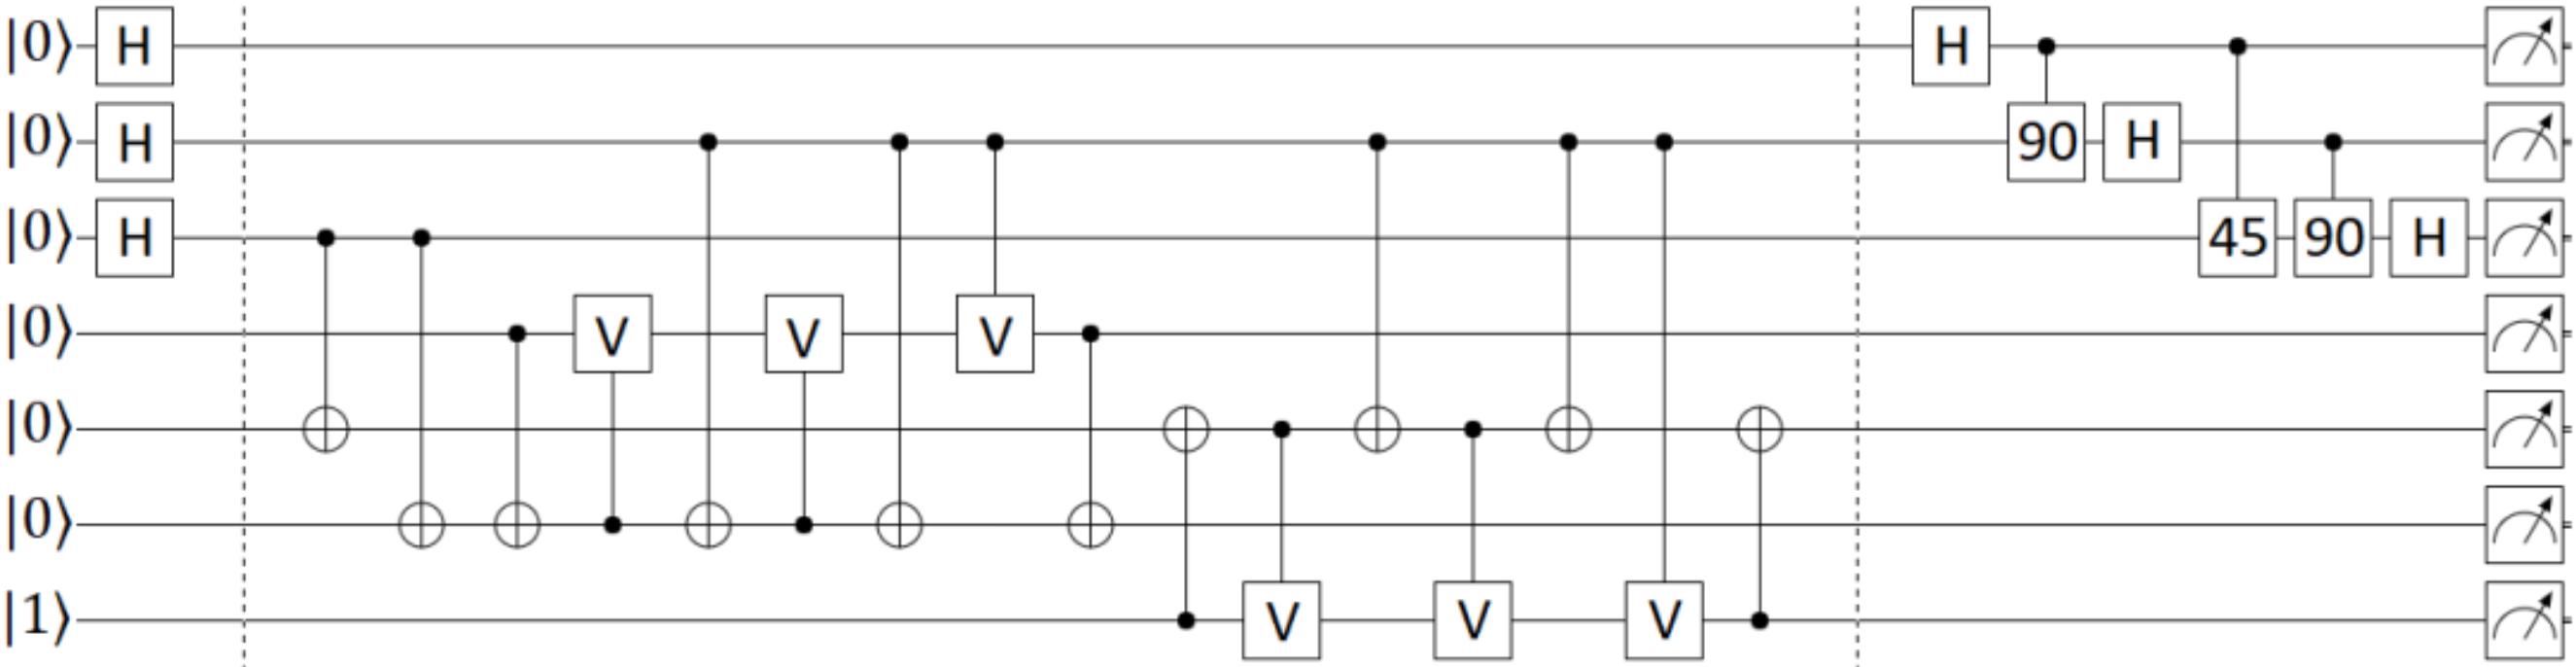
\includegraphics[width=0.7\textwidth]{shor_example.png}
  \caption{Esempio di algoritmo di Shor per fattorizzare il numero 15}
  \label{fig:shor_example}
\end{figure}

L'algoritmo di Shor si basa sulla teoria per la fattorizzazione dei numeri.

Supponiamo di voler fattorizzare un numero \(N\), l'algoritmo:

\begin{enumerate}
  \item Controlla se \(N\) è numero primo o potenza di un numero primo, attraverso l'utilizzo di un qualsiasi test di primalità che sia polinomiale, e se è così si ferma, altrimenti passa al punto numero 2;
  \item Sceglie un numero casuale \(a\) tale che \(1 < a < N\);
  \item Se \(b = mcd\left(a, N\right) > 1\), dove \(mcd\) può essere calcolato in tempo polinomiale utilizzando l'algoritmo di Euclide, restituisce \(b\) e si ferma, altrimenti passa al punto numero 4;
  \item Trova l'ordine \(a \% N\) tale che
    \[
      a^r \equiv 1 \% N \;\; con \; r > 0
    \]
  \item Se \(r\) è dispari torna al punto numero 2, altrimenti passa al punto numero 6;
  \item Calcola
  \[
    x = a^{\frac{r}{2}} + 1 \% N
  \]
  \[
    y = a^{\frac{r}{2}} - 1 \% N
  \]
  \item Se \(x = 0\), torna al punto numero 2;
  \item Se \(y = 0\), prende \(r=\frac{r}{2}\) e torna al punto numero 5;
  \item Calcola \(p = gcd(x,N)\) e \(q = gcd(y,N)\). Uno tra i due sarà fattore non banale di \(N\).
\end{enumerate}

L'algoritmo appena illustrato potrebbe essere svolto in tempo ottimale anche da un computer classico se non fosse per il punto 4 che è computazionalmente molto oneroso, quindi l'ideale è utilizzare un computer quantistico. In termini di tempo, l'algoritmo di Shor può fattorizzare un intero \(N\) in tempo \(O(\log^3 N)\) e in spazio \(O(\log N)\).

\subsubsection{Algoritmo di Shor e minacce sulla Blockchain}
La maggior parte dei sistemi crittografici a chiave pubblica possono essere rotti utilizzando questo algoritmo quantistico, che andrà semplicemente ad utilizzare un numero di qubit pari al doppio della dimensione della chiave. Per comprendere al meglio il problema, basta prendere in considerazione l'RSA 2048: un computer classico con una CPU da 5 Ghz impiegherebbe circa 13,7 miliardi di anni per decifrarne un codice mentre un computer quantistico con CPU da 10 Mhz sarebbe in grado di fare ciò in circa 42 minuti\cite{kearney2021vulnerability}.

Lo schema di crittografia asimmetrico Rivest Shamir Adleman (RSA), che consiste nello scambio di messaggi tramite utilizzo di una chiave pubblica, che li cifra, e una privata, che li decifra, è molto simile al metodo utilizzato dalle tecnologie Blockchain per la creazione e la crittografia di wallet di criptovalute. In questo caso, quindi, viene generata una coppia di chiavi: quella pubblica, utilizzata per ricevere criptovalute e consultare il saldo presente sulla Blockchain, e quella privata, utilizzata per spendere le criptovalute. Questo tipo di schema si basa quindi su funzioni matematiche \textit{one-way} e numeri primi, motivo per il quale, l'applicazione dell'algoritmo quantistico di Shor, porterebbe alla violazione della crittografia RSA, con chiave a 2048 bit, attraverso l'utilizzo di un computer quantistico a 4096 qubit logici.

\subsection{L'algoritmo di ricerca di Grover}
Ideato nel 1996 da Lov Grover, è un algoritmo di ricerca che, sfruttando l'amplificazione d'ampiezza, è in grado di cercare un elemento o un valore, in un insieme non ordinato, in tempo \(O\left(\sqrt{N}\right)\) a differenza degli algoritmi classici che risolvono lo stesso problema in tempo \(O\left(N\right)\).

\begin{figure}[h]
  \centering
  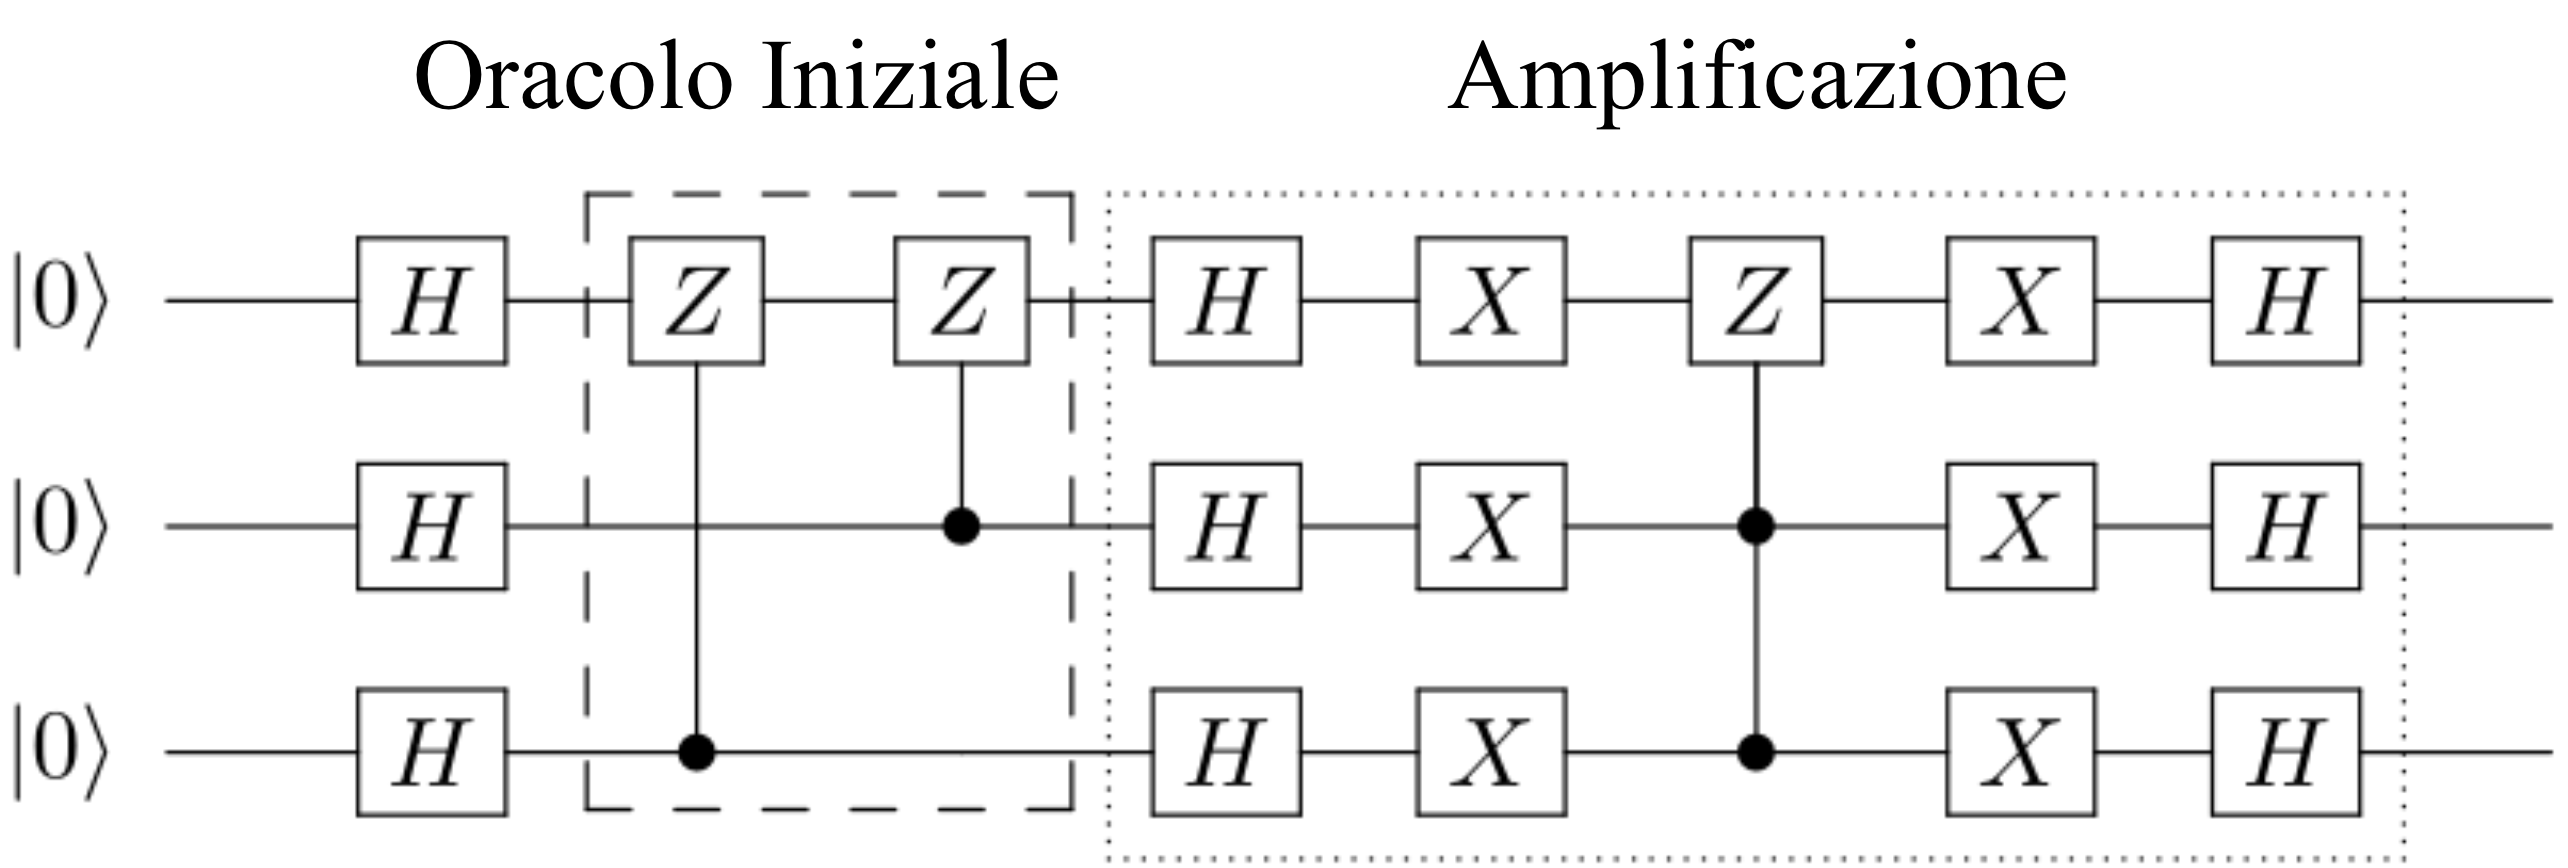
\includegraphics[width=0.7\textwidth]{grover_example.png}
  \caption{Esempio di algoritmo di Glover per 3 qubit}
  \label{fig:grover_example}
\end{figure}

\subsubsection{Algoritmo di Grover e minacce sulla Blockchain}
L'algoritmo di consenso della Blockchain, si basa sul calcolo di funzioni
crittografiche hash che, a partire da un input, genera una stringa di byte a lunghezza fissa. La produzione di transizioni hash, però, renderebbe la Blockchain sicura e non manomettibile se non fosse che, l'algoritmo di Grover permette di individuare, con poco sforzo computazionele, i dati originali su cui è stato applicato l'hash: ciò permette la generazione di collisioni hash più efficiente rispetto alla ricerca a forza bruta, che richiede invece tempo lineare.

Inoltre, c'è da sottolineare che, nonostante gli attacchi tramite algoritmo di Grover sono considerati meno rischiosi rispetto a quelli di Shor, non è noto un sistema PoW abbastanza resistente a tali attacchi mentre, nel secondo caso, è possibile sostituire la crittografia vulnerabile con una crittografia post-quantistica, permettendo quindi di affrontare al meglio le minacce ricevute.